\begin{doublespace}

\hyphenation{a-mong post-zy-got-ic wheth-er ac-cu-mu-lat-ed}

\chapter{Compensatory adaptation causes rapid incipient speciation}
\label{chap:comp_spp}

\section{Introduction}

Biological speciation is the evolution of reproductive isolating
barriers that prevent populations from interbreeding \citep{coy04}.
%
One potentially important barrier causes `intrinsic postzygotic isolation,'
in which hybrids are sterile or inviable from developmental, physiological,
or behavioral abnormalities \citep{coy04}.
%
Intrinsic postzygotic isolation is believed to commonly evolve
from genetic incompatibilities: negative epistatic interactions
among population-specific alleles inherited by the hybrids \citep{pre10}.
%
Alleles in a population may arise and spread by natural selection,
but the selective pressures involved are often unknown \citep{sch09}.
%
In order to infer the selective pressures that ultimately caused
population-specific alleles involved in genetic incompatibilities,
studies using methods in genetic mapping and molecular genetics
have helped identify `speciation genes' and their functions
\citep{noo06,mah11}.
%
Many of these genes involve the internal environment of the cell,
such as cellular housekeeping, genetic regulation, genetic conflict,
and coevolution between nuclear and mitochondrial genomes \citep{noo06,wol10}.
%
Interestingly, these genes often appear to have been driven
by natural selection \citep{noo06}, suggesting that adaptation to the internal,
genetic environment (as opposed to the external, ecological environment)
can lead to intrinsic postzygotic isolation \citep{pha09,pre10}.



One class of adaptation to the genetic environment
is compensatory adaptation, in which secondary mutations
compensate for the effects of accumulated deleterious mutations
\citep{har96,bur99,moo00,lev00,mai02,est03,est11}.
%
Deleterious mutations may accumulate in a population
through genetic drift \citep{lan94,lyn95},
hitchhiking with beneficial mutations \citep{chu11},
transient environmental changes \citep{bjo00},
or spread of selfish genetic elements \citep{pre10}.
%
Compensatory adaptation recovers and maintains the original phenotype
via stabilizing selection (i.e., selection against extreme phenotypes),
and thus leads to genotypic, not phenotypic, changes \citep{har96}.
%
Populations undergoing independent compensatory adaptation
will therefore diverge genetically, accumulating their own unique set
of deleterious and compensatory mutations.
%
Hybrids between such compensated populations would acquire
a mismatched set of deleterious and compensatory mutations,
exposing genetic incompatibilities that reduce hybrid fitness
\citep{har96,orr01,kon02,kul04,lan07,sch09b,pre10},
%
In this way, compensatory adaptation may lead to
intrinsic postzygotic isolation.



However, whether compensatory adaptation can lead to postzygotic isolation
remains to be tested experimentally.
%
Here I perform such an experiment to answer the following questions:
(1)~does postzygotic isolation evolve from independent compensatory adaptation?
(2)~what is the strength of genetic incompatibilities formed?
and (3)~what is the relative contribution of compensatory mutations
and deleterious mutations to postzygotic isolation?
%
Answering these questions requires that I identify
both deleterious and compensatory alleles,
which involves genetic manipulations that test the allelic
effects of each type of mutation.
%
For example, compensatory mutations must not be beneficial
in the absence of the deleterious mutations they compensate,
and thus they must be tested on their own.
%
Such genetic manipulations, however, are difficult even in
model systems, where genetic tools have been greatly advanced.



Therefore, I conducted my experiments using the artificial life system
Avida \citep{ofr04} (see p. \pageref{sec:avida}),
which has been used previously to study various questions
in evolution \citep{len99,len03,cho04,mis06,ele07,ele08,mis10}.
%
Avida has enabled research on evolving genetic systems
that would have been difficult in natural systems \citep{ada06},
and the similarities between digital and biological organisms
in many evolutionary phenomena have been remarkable \citep{wil02,ada06}.
%
Avida enhances the benefits of microbial systems
(i.e., short generation times, considerable replication,
easy manipulation and storage of genomes),
while being a true instance of evolution of a genetic system,
where the generality of evolutionary principles can be tested
\citep{len99,ele08,mis06}.
%
Specific to this study, Avida allowed us to easily insert deleterious mutations
of various effect sizes, carry out thousands of hybridizations,
and individually identify compensatory mutations.



Using Avida, I isolated mutants with deleterious mutations
from a well-adapted ancestor, and I allowed those mutants to evolve
in replicate for thousands of generations.
%
I then hybridized compensated populations and measured their fitness
to test for postzygotic isolation,
and I identified individual compensatory mutations to determine
their strength and contribution to postzygotic isolation.
%
I found that (1) postzygotic isolation occurred between compensated populations,
(2) the strength of incompatibility among compensatory mutations
was greater than among neutral mutations, and
(3) compensatory mutations contributed as much as deleterious mutation
to postzygotic isolation.
%
Our results suggest that compensatory adaptation may be an important
mechanism by which genetic incompatibilities and
thus intrinsic postzygotic isolation evolve.
%
Because I used a non-specific genetic system to test this hypothesis,
my results can be generalizable to biological organisms and motivate
future tests in biological organisms.



\section{Results}

Starting with a sexually-reproducing, haploid digital organism
that was not adapted to its environment but could replicate,
I allowed three independent populations to evolve
for about 250,000 generations under the same environmental configuration.
%
I used the most common genotype of each adapted population
as an independent ancestor for all subsequent experiments.
%
From the ancestors, I isolated 472 mutants
with 1-5 random irreversible mutations
whose combined negative fitness effect was either
small ($\Delta W$~=~0.01-0.1) or large ($\Delta W$~=~0.1-0.9).
%
As a control, I also isolated 74 neutral mutants ($\Delta W$~=~0.0)
with the same range of mutations per genome as those
in the small-effect and large-effect treatments (Table~\ref{tbl1}).
%
I then allowed populations founded by each mutant (including the controls)
to evolve for about 6,000 generations
in identical environmental conditions as their ancestor.
%
I regarded a population as compensated if its most common genotype
(1)~had a fitness at least equal to that that of its ancestor,
(2)~did not acquire mutations that were beneficial on their own, and
(3)~did not acquire mutations that were deleterious when they first appeared.



\begin{table}
\centering
\begin{tabular}{lccc}
Treatment & Ancestor & Mutants & Compensated \\
\hline
        & 1 & 25 & - \\
Neutral & 2 & 25 & - \\
        & 3 & 24 & - \\
\hline
        & 1 & 71  & 10 \\
Small   & 2 & 199 & 15 \\
        & 3 & 69  & 6  \\
\hline
        & 1 & 44  & 9 \\
Large   & 2 & 44  & 5 \\
        & 3 & 45  & 6 \\
\hline
\end{tabular}
\caption{Number of mutants and compensated populations per ancestor for
  the different treatments}
\label{tbl1}
\end{table}



\subsection{Reproductive isolation via compensation is rapid}

In nature, subpopulations that split off from their ancestral population may
come into secondary contact with their ancestor or with another subpopulation.
%
To model these two scenarios, I performed two types of hybridizations:
(1)~between compensated populations and their ancestor (`AC')
and (2)~between pairs of compensated populations (`CC').
%
I also performed these two types of hybridization on the control populations
(i.e., those that evolved starting with neutral mutations).
%
Note that these hybridizations were performed after all experimental evolution
had completed, i.e., populations evolved independently.
%
I found that the mean fitness of hybrids for both hybridization types
was lower than that of hybrids from control populations
(in Fig.~\ref{fig1}, compare `Control' hybrids with `Del.~+~Comp.' hybrids).
%
Surprisingly, whether populations compensated for
small- or large-effect deleterious mutations
did not have a significant effect on mean hybrid fitness
(in Fig.~\ref{fig1}, the 95\% bootstrap confidence intervals overlap for
`Small-effect Del.~+~Comp.' and `Large-effect Del.~+~Comp.').
%
These findings show that intrinsic postzygotic isolation developed faster
during compensatory adaptation than during neutral evolution,
regardless of the fitness effect size of the initial deleterious mutations.



\begin{figure}
\centering
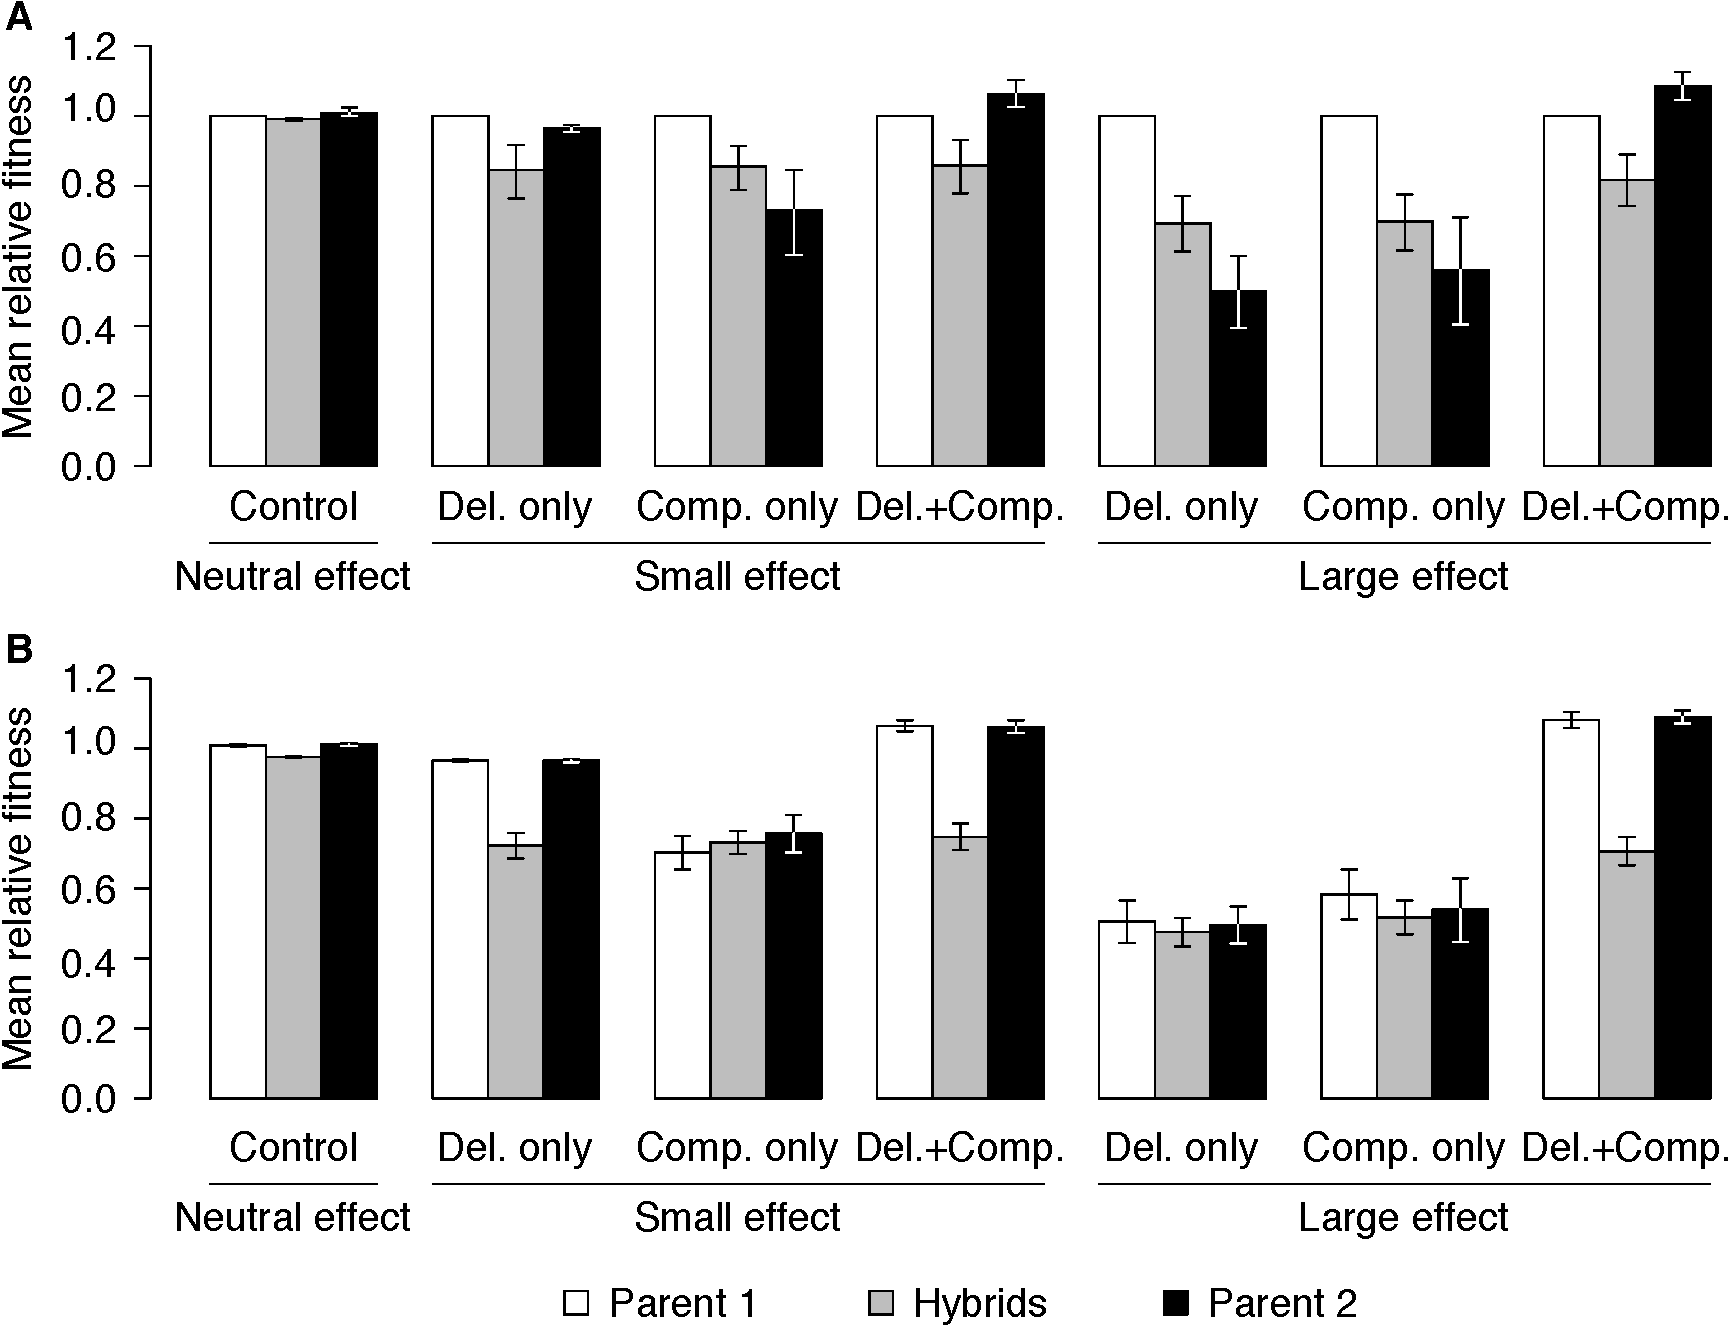
\includegraphics[width=\linewidth]{fig1.pdf}
\caption{Fitness of hybrids after 25,000 updates of parental evolution.
  Populations compensated for either small-effect or large-effect
  deleterious mutations.
  (A) Hybridizations between compensated genotypes and their ancestor.
  (B) Hybridizations between pairs of compensated genotypes
  sharing the same ancestor.
  `Del. Alone' include only the initial deleterious mutations
  before compensation,
  `Comp. Alone' include only the compensatory mutations after compensation,
  and `Del. + Comp.' include both deleterious and compensatory mutations.
  `Control' include all mutations accumulated neutrally.
  Error bars are 95\% bootstrap confidence intervals.}
\label{fig1}
\end{figure}



\subsection{Compensatory adaptation forms strong genetic incompatibilities}

Compensated populations acquired 2-10 mutations at the end of the runs,
while control populations acquired only 0-1 mutations.
%
Compensated populations thus had greater potential for creating
a greater number of genetic incompatibilities than control populations.
%
To determine whether compensated populations created stronger
genetic incompatibilities than control populations,
I accounted for the number of mutations acquired by each type of population.
%
If hybrids between compensated genotypes
have stronger genetic incompatibilities
than hybrids between control genotypes,
then the rate at which hybrid fitness decays
with the number of inherited mutations
should be greater for hybrids between compensated genotypes
than for hybrids between control genotypes.
%
In other words, the slope of the line relating
the number of mutations in hybrids
with the hybrid fitness should be greater
for hybrids between compensated genotypes
than for hybrids between control genotypes.



Before I performed this test, however,
I generated a new set of 250 control genotypes
because my experimental control populations
acquired only 0-1 mutations after about 6,000 generations.
%
To generate the new control genotypes,
I introduced 2-10 neutral mutations into ancestral genotypes,
which was within the range of number of mutations in compensated genotypes.
%
I then fit a least squares linear relationship between
the mean number of mutations in hybrids
and the hybrid fitness for each treatment
(i.e., neutral-, small-, and large-effect for both AC and CC hybrids).
%
I found that the slope of this linear relationship
was significantly greater for hybrids between compensated genotypes
than for hybrids between control genotypes (Fig.~\ref{fig2}B),
but was not significantly greater for AC hybrids (Fig.~\ref{fig2}A).
%
Our findings suggest that genetic incompatibilities
involving deleterious and compensatory mutations in hybrids
were stronger than those among neutral mutations.



\begin{figure}
\centering
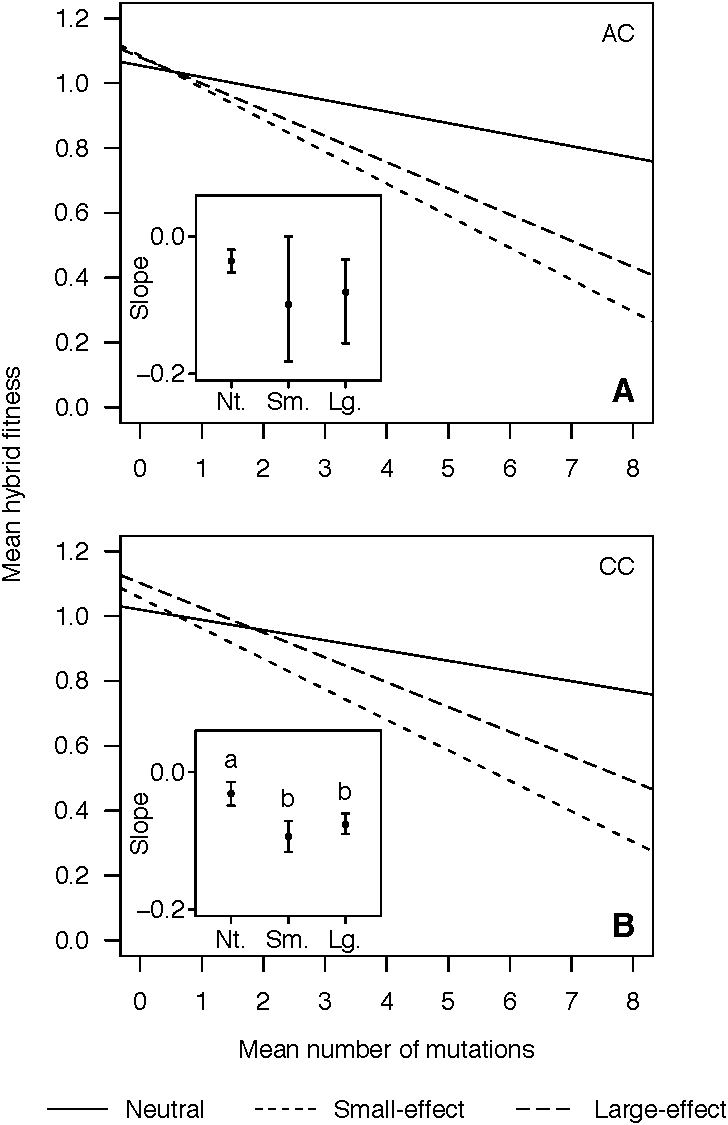
\includegraphics[width=\linewidth]{fig2.pdf}
\caption{Strength of genetic incompatibilities in hybrids.
  (A) Least squares linear fit of the mean number of mutations in hybrids
  between ancestor and compensated genotypes (AC) against their mean fitness.
  (B) Same as (A) except for hybrids between pairs of compensated genotypes
  (CC). Insets: Means and 95\% bootstrap confidence intervals of each slope
  where shared letters indicate overlapping confidence intervals.}
\label{fig2}
\end{figure}



\subsection{Both deleterious and compensatory mutations
  contribute to reproductive isolation}

Although I have shown that genetic interactions
involving deleterious and compensatory mutations
may form strong genetic incompatibilities rapidly,
I have yet to quantify the relative contributions
of each type of mutation to the formation of genetic incompatibilities.
%
At first glance, Fig.~\ref{fig1}
may suggest that compensatory mutations
contributed little to reproductive isolation
because hybrids between genotypes before compensation (`Del.~only')
had fitnesses as low as hybrids after compensation (`Del.~+~Comp.').
%
However, hybrids between compensated genotypes in which deleterious mutations
were reverted to the ancestral state also had low fitnesses
(in Fig.~\ref{fig1}, compare `Comp.~only' hybrids to `Del.~+~Comp.' hybrids),
suggesting that compensatory mutations
also contributed to postzygotic isolation.



To establish more directly the extent to which incomplete sets
of deleterious and their corresponding compensatory mutations
contributed to postzygotic isolation,
I generated genotypes with different proportions
of deleterious and compensatory mutations.
%
I generated such genotypes by creating every possible hybrid
between a compensated genotype and its ancestor.
%
For each genotype, I then measured its fitness and calculated
the proportion of deleterious and compensatory mutations
relative to the compensated parental genotype.
%
I performed this analysis on all compensated genotypes
for both the small-effect and large-effect treatments.
%
I found that, unless genotypes contained either
all or none of their parent's deleterious and compensatory mutations,
their fitness was low (Fig.~\ref{fig3}),
suggesting that both deleterious and compensatory mutations
contributed to postzygotic reproductive isolation.



\begin{figure}
\centering
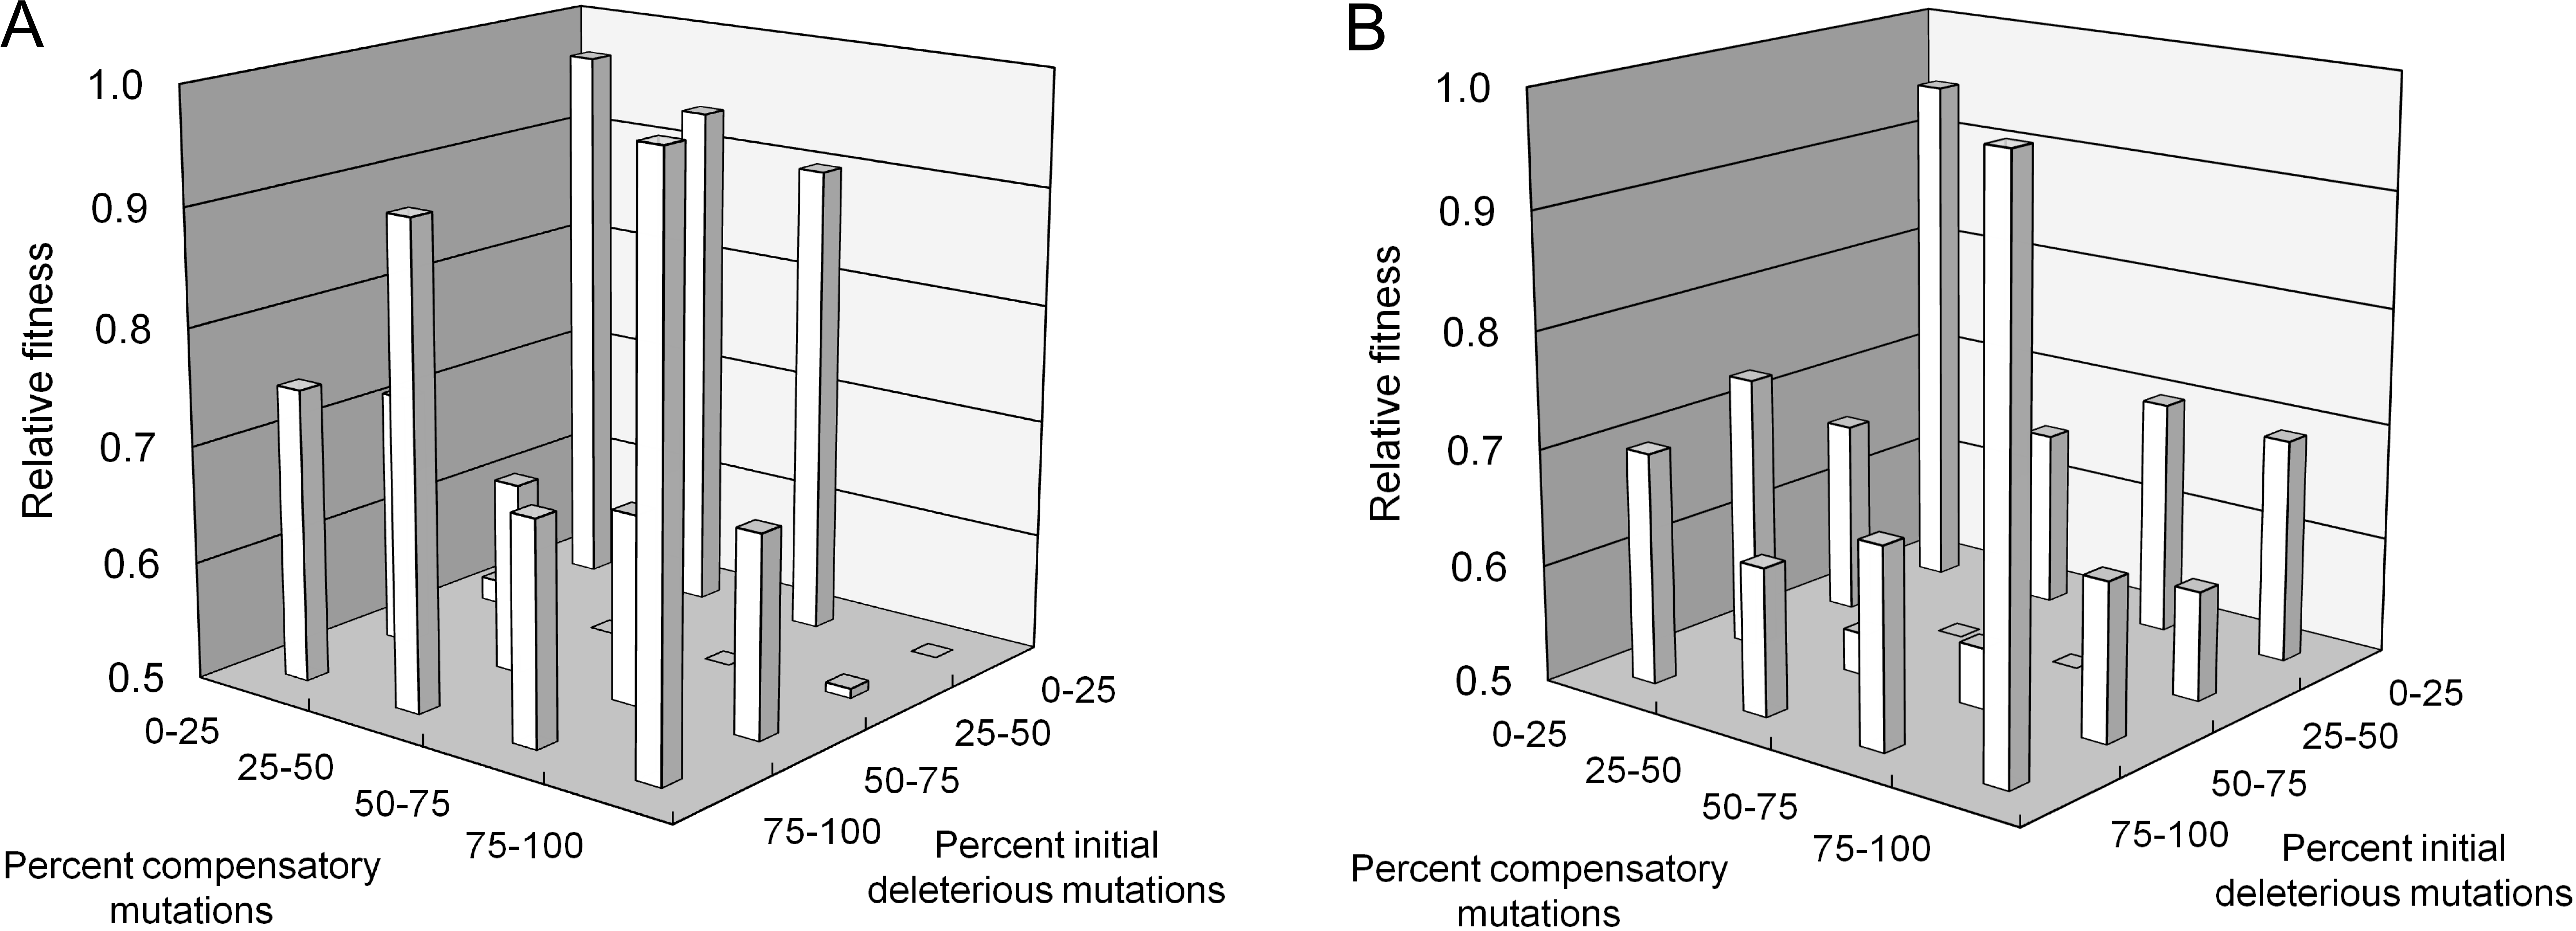
\includegraphics[width=\linewidth]{fig3.png}
\caption{Fitness of hybrids with intermediate parental contributions
  of deleterious and compensatory mutations.
  (A) Mean fitness of hybrids between the ancestor
  and compensated parents that inherit the specified percent of small-effect
  deleterious and compensatory mutations. (B) Same as (A) except for
  large-effect deleterious mutations.}
\label{fig3}
\end{figure}



\section{Discussion}

Most genes involved in intrinsic postzygotic isolation,
i.e., hybrid sterility or inviability
due to developmental or physiological abnormalities,
show strong signatures of positive selection \citep{pre10}.
%
Surprisingly, many of these genes
are not adaptations to the external, ecological environment
but to an impaired internal, genetic environment
(see Table~\ref{tbl1} in \citep{pre10}).
%
An example of adaptation to an impaired genetic environment
is adaptive compensation of deleterious mutations
\citep{har96,bur99,moo00,lev00,mai02,est03,est11}.
%
Populations undergoing independent compensatory adaptation
will diverge genetically
and may form genetic incompatibilities,
causing intrinsic postzygotic isolation
\citep{orr01,kon02,kul04,coy04,lan07,sch09b,pre10}.
%
Under this scenario, I asked:
how rapidly does postzygotic isolation evolve?
what is the strength of genetic incompatibilities?
and what are the relative contributions
of compensatory and deleterious mutations to isolation?



Using an artificial life system,
I found that postzygotic isolation
due to compensation was rapid:
hybrids between compensated populations
had significantly lower fitness
than hybrids between populations that did not undergo compensation,
regardless of the effect size
of the initial deleterious mutations.
%
I also found that compensatory adaptation
formed stronger genetic incompatibilities:
the rate at which hybrid fitness
decayed with the number of mutations
was significantly greater
for hybrids between compensated populations.
%
Finally, I found that both
deleterious and compensatory mutations
contributed to postzygotic isolation:
hybrids with different proportions
of compensatory and deleterious mutations
were unfit unless all or none
of both types of mutations were present.



Two important implications to the genetics of postzygotic isolation
can be drawn from my findings.
%
First, evidence of genotypic diversification between species
may not correlate with phenotypic diversification.
%
This is because compensatory adaptation can build up genetic differences
without altering phenotypic characteristics.
%
In fact, compensatory adaptation may act under stabilizing selection
to maintain phenotypes despite continual accumulation of
deleterious mutations \citep{har96}.
%
Second, evidence of positive selection
at loci that contribute to speciation (`speciation genes')
may not always be the result of diversification
due to ecological adaptation
but instead be the footprint of compensatory adaptation.
%
Our results corroborate the view that
adaptation to the internal, genetic environment
may be important in the development
of intrinsic postzygotic isolation \citep{pre10,pha09}.



In describing his mechanism of founder speciation, Ernst Mayr stated that
``\dots\ the mere change of the genetic environment may change the
selective value of a gene very considerably'' \citep{tem08}.
%
In cases where founder events cause the fixation or high frequency
of deleterious mutations, compensatory adaptation may provide a
mechanism by which genes with altered selective values change
in allele frequency.
%
Furthermore, Templeton's model of genetic transilience recognizes
that founder populations may be affected by genetic drift
while new mutations and recombination increase genetic variation \citep{tem08}.
%
Genetic drift alone can raise the frequency of deleterious mutations
in a founder population while increased genetic variation
may introduce new compensatory mutations on which selection can act.
%
Our study using experimental evolution with populations of digital organisms
suggests that such compensatory mutations can rapidly generate
postzygotic barriers, and therefore supports a novel genetic mechanism
for models of founder or peripatric speciation.
% Check out paper:
% Increased mitochondrial mutation frequency after an island colonization: positive selection or accumulation of slightly deleterious mutations?


Our study took advantage
of the recent implementation of sexual reproduction
in the artificial life platform Avida \citep{mis06},
and extended its application
as proof of principle to the field of speciation.
%
I demonstrated that Avida is a useful tool to complement
other approaches in speciation research as it allows for
the direct observation of evolution and reproductive isolation in action.
%
Furthermore, my conclusions will motivate additional research
into compensatory adaptation as a viable mechanism for speciation,
to be further explored in biological systems.
%
The notion that organisms construct or choose
their own microhabitats \citep{lew00}
suggests that organisms are somewhat
resilient to changes in the external environment.
%
This reduced emphasis on the external environment in evolution
is supported by my conclusion that environmental differences
between allopatric populations are not essential for genetic diversification.



\section{Materials and Methods}

\subsection{Strains and experimental conditions}

The starting digital organism I used was the `default' sexually-reproducing
organism in Avida, with a genome length fixed to 80 instructions.
%
The population size was set to 10,000 organisms,
and the copy mutation probability was set to 0.0005 per instruction
(i.e., 0.04 per genome per generation).
%
Other types of mutations, such as insertions or duplications,
were not permitted because they may disrupt homologous recombination.
%
Digital organisms were configured to reproduce sexually,
and the two recombinant offspring were set to replace random individuals
in the population when no free space was available.
%
The `diverse' environment rewarded the nine tasks
commonly used in Avida experiments \citep{len03}.
%
The small genome size of digital organisms caused reversions
to be common during compensatory adaptation in preliminary runs.
%
To guarantee that genotypic changes were due to mutations at secondary loci%
---as has been observed in biological organisms \citep{bur99,est11}---%
I prevented reversions from occurring.



\subsection{Isolation of mutants}

To generate mutants for the small-effect and large-effect treatments,
I first generated sets of 10,000 random mutant genotypes
for each evolved ancestor until either four mutants
with the desired number of mutations and effect size were found,
or until 100 million mutants had been searched.
%
For the small-effect treatment, effect sizes of
0.01, 0.02, 0.03, 0.04, 0.05, 0.06, 0.07, 0.08, 0.09, and 0.1
(each with up to a 0.0049 deviation) were identified for genotypes carrying
1, 2, 3, 4, or 5 mutations.
%
For the large-effect treatment, mutants with effect sizes of
0.1, 0.2, 0.3, 0.4, 0.5, 0.6, 0.8, and 0.9 (with up to a 0.049 deviation)
for each mutation number of 1, 2, 3, 4, and 5 were identified.
%
(Effect size is the difference between
the fitnesses of the ancestral and the mutated genotype,
relative to the ancestral genotype.)
%
I isolated a total of 339 small-effect mutants
(after running the above procedure twice) and 133 large-effect mutants.
%
I implemented a different searching procedure for neutral mutations
because the probability of several random mutations resulting
in a neutral genotype was very low.
%
To find neutral mutants, I first generated 10,000 single-mutants
and selected the first one that was neutral
(i.e., relative fitness of exactly 1.0).
%
This procedure was repeated starting with the neutral mutant until
the desired number of mutations was reached or until the
recursion was exhausted.
%
I isolated a total of 74 neutral mutants.



\subsection{Compensated populations}

I regarded a population as compensated if its most common genotype
(1)~reached a fitness of at least 1.0 relative to its ancestor,
(2)~did not acquire mutations that were beneficial on their own, and
(3)~did not acquire mutations that were deleterious when they first appeared.
%
To determine condition (1), the most common genotype at the end of a run
was isolated and its fitness relative to its ancestor was measured.
%
If its relative fitness was equal to or greater than 1.0,
then the population was considered compensated.
%
To determine condition (2), the fitness effect of each
secondary mutation in the most common genotype of the population
was tested in the genetic background of the ancestor.
%
If any `transformant' had a relative fitness above 1.0,
then that population was not considered as compensated
because mutations were beneficial on their own
(i.e., generally beneficial, not compensatory);
otherwise, the population was considered compensated.
%
To determine condition (3), I sequentially examined the
most common genotype of the population about every three generations.
%
If the gain of any mutation resulted in a lower fitness than the
genotype at the previous third generation,
then that population was not considered as compensated;
otherwise, the population was considered compensated.



\subsection{Hybridization method}

Hybrids were created by the same method in which Avida
creates recombinants during sexual reproduction:
the genetic region between two crossover points
were exchanged between two parents to produce two offspring.
%
Hybridizations, whether between compensated populations
and their ancestor or between pairs of compensated populations,
involved creating every possible hybrid
between the most common genotypes of each population.



\subsection{Statistics}

To compare the fitness of hybrids among treatments (Fig.~\ref{fig1}),
I determined whether their 95\% bootstrap confidence intervals overlapped.
%
For each treatment, bootstrap replicates were set to contain the
same number of samples per ancestor---established as the mean number
of observed samples per ancestor---in order to minimize any
potential bias from the fact that ancestors yielded different
numbers of compensated populations.
%
All bootstraps contained 10,000 replicates.
%
To determine the linear relationship between the number of mutations
in hybrids and their fitness (Fig.~\ref{fig2}),
I fit a linear least squares model to each bootstrap replicate.
%
I compared the 95\% bootstrap confidence intervals of the slopes
among treatments to establish the relative effect of mutation number
on hybrid fitness.
%
Statistical analyses were performed in R (ver.~2.8.1).



\section{Acknowledgments}

I thank R. E. Lenski, D. W. Schemske, and C. Ofria, I. Dworkin,
and A. Gerstein for helpful discussion and comments on the manuscripts.
%
This work was supported by the Quantitative
Biology Initiative at Michigan State University (MSU)
and the BEACON Center for the Study of Evolution in Action.
%
Computational experiments were made possible by the
High Performance Computing Center at MSU.
%
This material is based in part upon work supported
by the National Science Foundation under Cooperative Agreement No. DBI-0939454.
Any opinions, findings, and conclusions or recommendations
expressed in this material are those of the authors
and do not necessarily reflect the views of the National Science Foundation.

\end{doublespace}

\bibliographystyle{apalike}
\bibliography{comp_spp}
